\section{Introdução}\label{sec:intro}


Sistemas de logística interna em centros de distribuição modernos (Fig.~\ref{fig:mercado_livre}) dependem fortemente de linhas automatizadas para transporte e separação de itens, permitindo maior eficiência na preparação de pedidos e redução da intervenção humana. Empresas como Amazon e Mercado Livre utilizam sistemas altamente integrados compostos por esteiras, sensores e robôs, capazes de identificar, rastrear e direcionar produtos em tempo real ao longo de múltiplos estágios do processo logístico. No processo de gestão de estoques da Amazon [1] e do mercado livre [2] são utilizados diversos sistemas embarcados de logística industrial, onde é possível observar a importância de tais sistemas no chão de fábrica [6]-[9], e a tendência é que haja uma ampliação desses sistemas de logística robotizados [5] para suprir a demanda de entregas e rastreamentos do mundo inteiro. Nesse contexto, módulos de esteiras desempenham papel fundamental como unidades básicas de movimentação e roteamento de itens dentro de arquiteturas modulares e escaláveis.

% Imagem de um Centro de distribuição (cajamar)
\begin{figure}[!htpb]
    \centering
    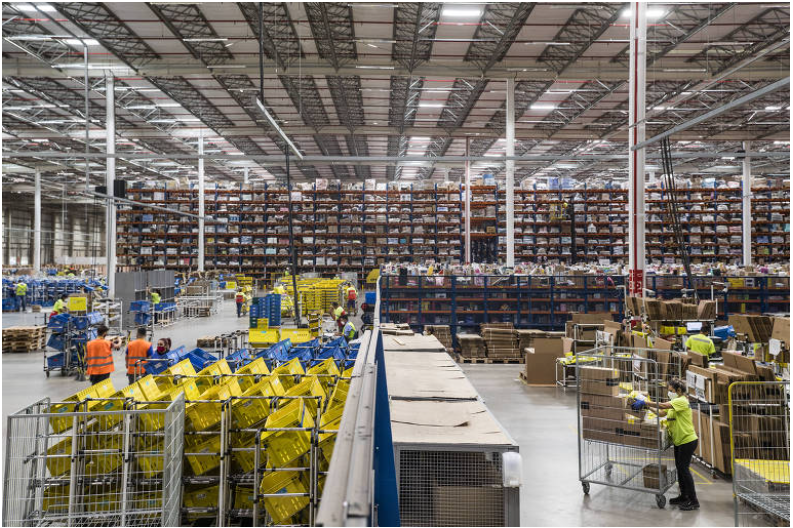
\includegraphics[width=0.75\linewidth]{figuras/centro_de_distribuicao_mercado_livre.png}
    \caption{Centro de distribuição do Mercado Livre em Cajamar, São Paulo.}
    \label{fig:mercado_livre}
\end{figure}


O problema central abordado neste trabalho consiste no desenvolvimento de um módulo de esteira automatizado capaz de reproduzir, em escala reduzida, o comportamento esperado de um sistema de separação de itens em uma linha de produção. Considera-se um fluxo contínuo de objetos, sendo necessário detectar sua presença, realizar a identificação do destino de cada objeto por meio da leitura de um código QR que acompanha o objeto e direcioná-los corretamente para diferentes saídas. Esse problema envolve desafios típicos de sistemas embarcados, como controle em tempo real, integração entre sensores e atuadores, comunicação com sistemas externos e divisão eficiente de tarefas entre diferentes níveis de processamento. 


No estado da arte, soluções industriais empregam arquiteturas distribuídas e altamente escaláveis, nas quais o processamento é dividido entre controladores de baixo nível responsáveis pelo gerenciamento do sistema mecatrônico em tempo real, e sistemas de alto nível, responsáveis por visão computacional, tomada de decisão e integração com sistemas de gestão. No meio acadêmico, diversos trabalhos exploram sistemas de separação automatizada baseados em visão computacional, identificação por código de barras ou QR code e controle embarcado de esteiras, frequentemente utilizando plataformas como microcontroladores e computadores de placa única (\textit{Single Board Computers – SBCs}) (Fig.~\ref{fig:rpi3}) para prototipagem e validação experimental. Entretanto, muitas dessas abordagens focam isoladamente na identificação ou no controle, não explorando de forma integrada a comunicação eficiente entre camadas de processamento com restrições reais de \textit{hardware}. Diante desse cenário, torna-se relevante o desenvolvimento de um protótipo acadêmico que permita explorar, de forma controlada, os principais desafios envolvidos na integração entre controle embarcado e processamento de alto nível, sem a complexidade e o custo associados a sistemas industriais completos.

%colocar imagem de um raspberry pi 3
\begin{figure}[!htpb]
    \centering
    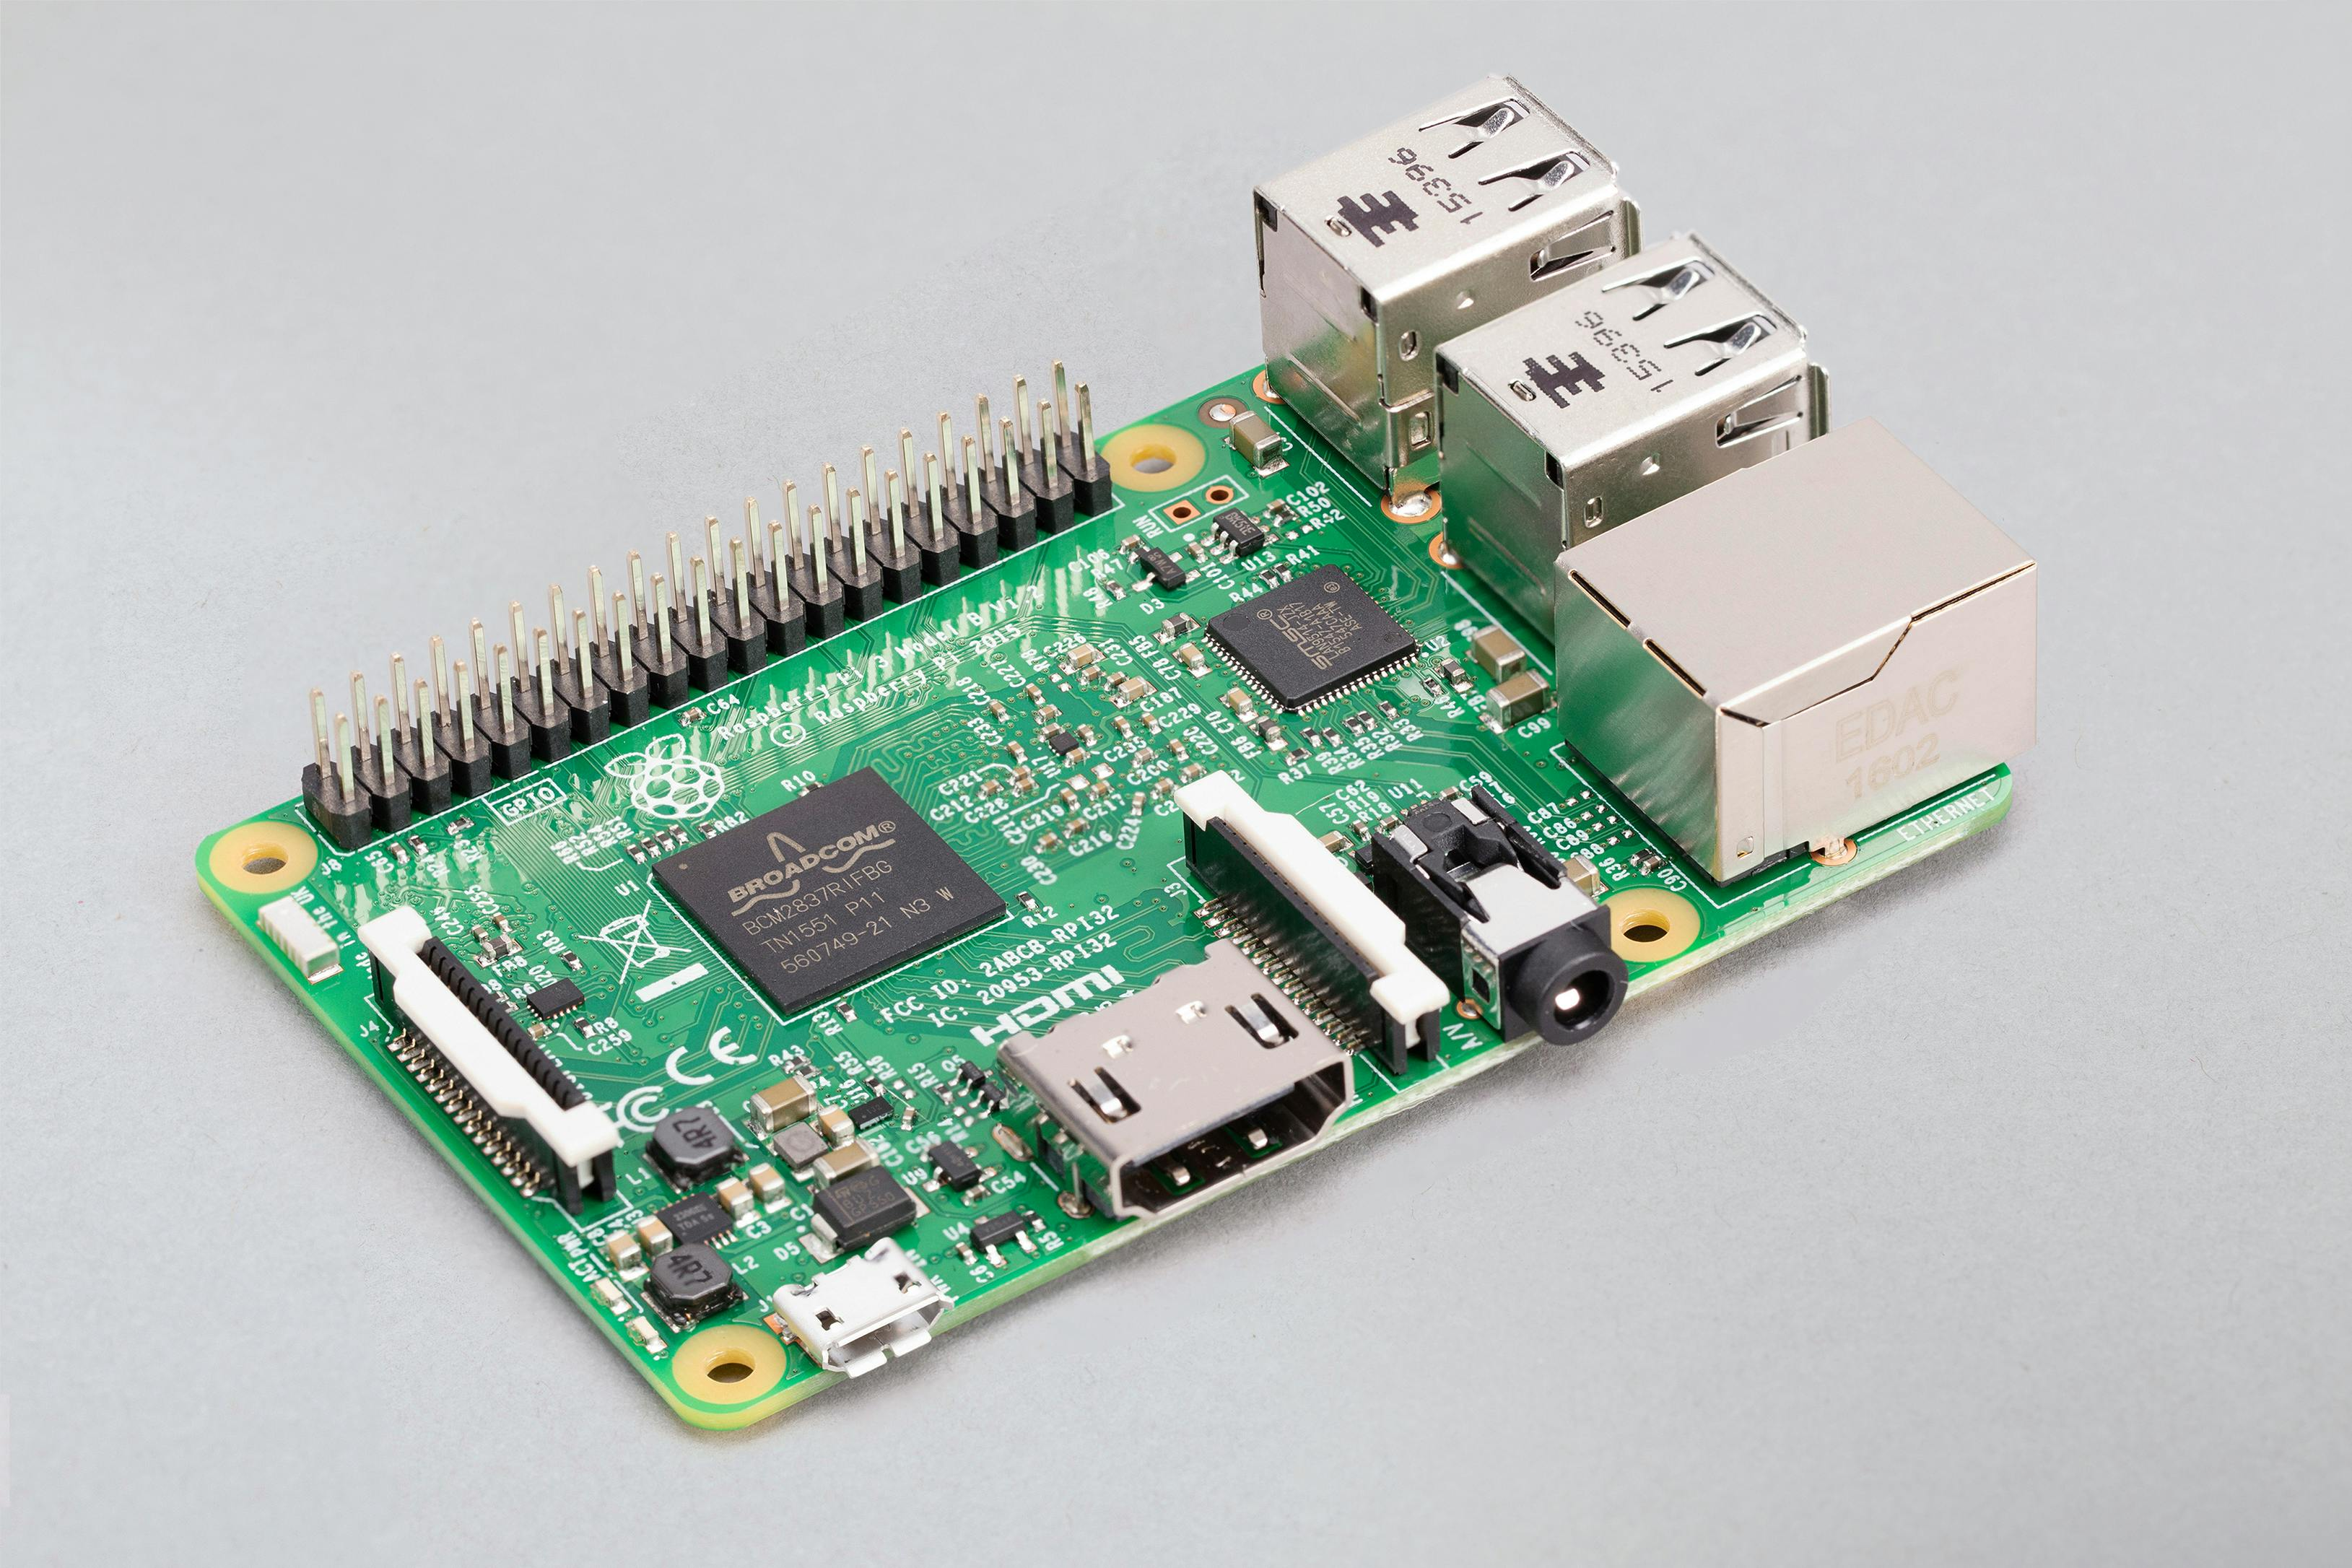
\includegraphics[width=.9\columnwidth]{figuras/rpi3.jpg}
    \caption{Raspberry Pi 3 Modelo B.}
    \label{fig:rpi3}
\end{figure}

Dessa forma, o presente trabalho propõe o desenvolvimento de um sistema embarcado para controle de um módulo de esteira automatizada em escala reduzida com uma entrada e duas saídas, capaz de realizar a separação de itens com base em decisões externas previamente associadas a um código QR de identificação do objeto. A arquitetura adotada diferencia-se por utilizar uma abordagem de processamento distribuído, na qual uma unidade de controle baseada em microcontrolador é responsável pelas tarefas de tempo real, enquanto um \textit{Single Board Computer} executando Linux embarcado realiza tarefas de mais alto nível, como captura de imagem, leitura de código QR, definição de destino e supervisão do sistema.


O sistema proposto tem como objetivo principal implementar um módulo funcional de separação de itens, capaz de detectar objetos, posicioná-los em uma zona de leitura, solicitar a identificação ao servidor Linux e executar o desvio para uma entre duas saídas possíveis. Para isso, são estabelecidos requisitos como a operação com objetos de pequeno porte (massa de até 250 g, volume máximo de 125 cm³ e altura entre 2 cm e 5 cm), o processamento sequencial de itens, a comunicação confiável entre o módulo embarcado e o servidor supervisor, e a execução determinística das ações de controle.

Como resultado esperado, busca-se a validação experimental de um protótipo funcional que demonstre a viabilidade da integração entre controle embarcado em tempo real e processamento de alto nível em ambiente Linux embarcado. A solução proposta também se destaca por seu caráter modular e didático, podendo servir como base para expansão em sistemas maiores de automação logística. Os arquivos do projeto estão disponíveis em repositório online (GitHub) por meio do link disponibilizado nas referências bibliográficas \cite{ref:github_soe}.